\documentclass[12pt]{article}

% For Different Coloured Comments
\usepackage{xcolor}

% For better title formatting
\usepackage{titling}

% For version history
\usepackage{vhistory}

% For references
\usepackage{hyperref}

\usepackage{indentfirst}

\usepackage{graphicx}

% To stop tables from being stupid
\usepackage{float}
\restylefloat{table}
\restylefloat{figure}

\setlength{\droptitle}{-10em}

%% Comments
\newif\ifcomments\commentstrue

% Comment Formatting
\ifcomments
\newcommand{\authornote}[3]{\textcolor{#1}{[#3 ---#2]}}
\newcommand{\todo}[1]{\textcolor{red}{[TODO: #1]}}
\else
\newcommand{\authornote}[3]{}
\newcommand{\todo}[1]{}
\fi

% Comment Colours
\newcommand{\wss}[1]{\authornote{magenta}{SS}{#1}}
\newcommand{\hm}[1]{\authornote{blue}{HM}{#1}} %Hediyeh
\newcommand{\tz}[1]{\authornote{blue}{TZ}{#1}} %Tahereh
\newcommand{\pl}[1]{\authornote{blue}{PL}{#1}} %Peng

% Spacing
\setlength{\parindent}{4em}
\setlength{\parskip}{1em}

\begin{document}

% Make the title
\title{Design Document for Knaves NES}
\date{\today\\
	{\medskip\small Software Engineering 3XA3, Lab \#3}
}
\author{Niko Savas\\
	\texttt{1300247}
	\and
	Joe Crozier\\
	\texttt{1311502}
	\and
	Sam Nalwa\\
	\texttt{1332792}
}

\maketitle
\clearpage

\tableofcontents
\clearpage

\section{Introduction}

KnavesNES is a software project which aims to emulate an MOS Technology 6502 CPU, as found in the popular Nintendo Entertainment System. The emulated CPU is able to perform all operations performed by the physical CPU and reads and manipulates from its own space of virtual memory. KnavesNES is programmed entirely in C++ using SDL and Visual Studio 2015. The choice to use C++ was that of optimization, as C++ is an exceptionally fast systems programming language. KnavesNES employs several object oriented programming principles, namely inheritance, modularity, and single class responsibility. 

This document aims to explain and deconstruct the various modules used by KnavesNES. While SRS was used to identify what was to be done by the software, the design document will instead explain how the requirements be accomplished. 

Included in this document is a module hierarchy of the behavior hiding process, a traceability matrix between modules and requirements, and a definition and explanation of each module.

\section{Anticipated and Unlikely Changes}
	\subsection{Anticipated Changes}
		\textbf{AC1} - The specific hardware on which KnavesNES is running.

		\textbf{AC2} - The length and content of the passed ROM file.

		\textbf{AC3} - The intermittent and final memory states.

	\subsection{Unlikely Changes}
		\textbf{UC1} - The passed ROM files will be encoded as machine code instructions.

		\textbf{UC2} - The instruction set of the CPU will be identical to that of the 6502.

		\textbf{UC3} - Memory will be outputted as ASCII encoded .log files.

		\textbf{UC4} - The size of the emulated memory will be that of the NES

		\textbf{UC5} - KnavesNES will be manipulated solely through the command line.

\section{Module Heirarchy}
	Because the Knaves NES emulator is simply emulating the CPU of an NES, it doesn't require significant module depth. In the larger scope of an NES emulator, the modules included in the CPU emulator would be lower level modules to the general emulator. For this reason, Knaves NES heirarchy is relatively flat, including only one Level 1 module.

		\textbf{M1: } Command Line Interfacing Module

		\textbf{M2: } CPU Module

		\textbf{M3: } Cartridge Module

		\textbf{M4: } Memory Module

	\begin{table}[H]
		\centering
		\begin{tabular}{p{2in} p{2in}}
			\hline
			Level 1 & Level 2\\
			\hline
			Command Line Interfacing Module & CPU Module\\
			- & Cartridge Module\\
			- & Memory Module \\
		\end{tabular}
		\caption{Module Heirarchy for Knaves NES}
	\end{table}	

\section{Connection Between Requirements and Design}
	\begin{table}[H]
		\centering
		\begin{tabular}{p{2in} p{2in}}
			\hline
			\textbf{AC} & \textbf{Modules} \\
			\hline
			AC1 & M1, M2 \\
			AC2 & M2, M3 \\
			AC3 & M2, M4 \\
		\end{tabular}
		\caption{Connections between Requirements and Design for Knaves NES}
	\end{table}

\section{Module Decomposition}
	\subsection{Command Line Interfacing Module}
		\textbf{Secrets: } The instances of the other modules, the CPU loop.

		\textbf{Services: } Controls the running of the Knaves NES. This is the entry point from the command line which will interface with the other modules in Knaves NES.

		\textbf{Implemented By: } Knaves NES

	\subsection{CPU Module}
		\textbf{Secrets: } CPU Registers getters/setters, Instruction Functions, means in which to execute instructions
		
		\textbf{Hidden information: } CPU status flags, CPU registers, program counter, 
		
		\textbf{Services: } Controls the execution of instructions. Reads an instruction from memory using the program counter register

		\textbf{Implemented By: } Knaves NES

	\subsection{Cartridge Module}
		\textbf{Secrets: } Means of reading instructions from cartridge and the position in which to store them in memory.

		\textbf{Hidden information: } Hexadecimal values of opcodes in ROM file.

		\textbf{Services: } Reads instructions from a ROM file, converts them to chars, then writes them to the necessary locations in memory.

		\textbf{Implemented By: } Knaves NES

	\subsection{Memory Module}
		\textbf{Secrets: } Reading and writing memory, outputting memory to log files

		\textbf{Hidden Information: } Current values stored in memory

		\textbf{Services: } Reads and writes values to and from memory, logs current state of memory

		\textbf{Implemented By: } Knaves NES

\section{Traceability Matrix}
	\begin{table}[H]
		\centering
		\begin{tabular}{ p{2in} p{2in} }
			\hline
			\textbf{Label} & \textbf{Description} \\
			\hline
			R1 & Knaves NES must be able to run standard NES ROMs (.nes files) \\
			R2 & Knaves NES CPU must be able to execute opcodes from the 6502 MOS CPU architecture\\
			R3 & Knaves NES CPU must be able to manage 2kB of RAM\\
			R4 & Knaves NES will log its memory state into a .log file in the user’s working directory at a specified interval.\\
		\end{tabular}
		\caption{Original Requirements for Knaves NES (Included in Requirements document, inserted here for reference.)}
	\end{table}

	\begin{table}[H]
		\centering
		\begin{tabular}{ p{2in}  p{2in} }
			\hline
			\textbf{Req.} & \textbf{Modules} \\
			\hline
			R1 & M1, M2, M3, M4\\
			R2 & M2, M4\\
			R3 & M2, M4\\
			R4 & M4\\
		\end{tabular}
		\caption{Traceability Matrix for Knaves NES}
	\end{table}



\section{Use Hierarchy Between Modules}
	\begin{figure}[H]
		\centering
		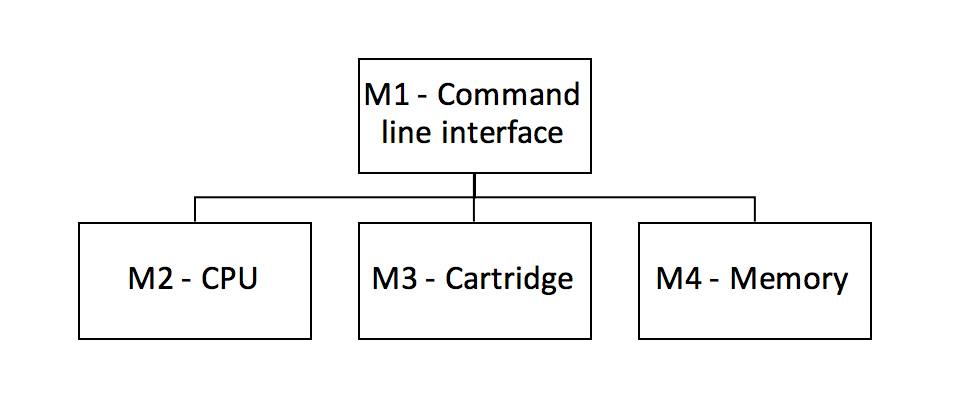
\includegraphics[width=90mm]{trace.jpg}
		\caption{Use Heirarchy Among Modules}
	\end{figure}

\section{Project Timeline}
	\begin{figure}[H]
		\centering
		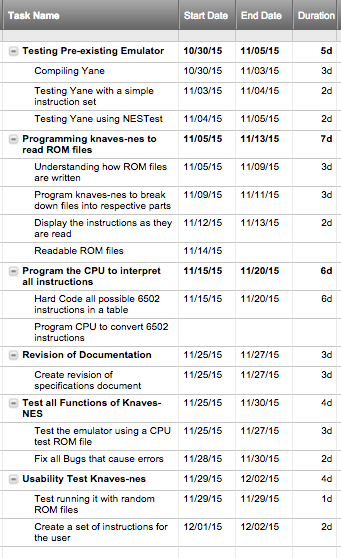
\includegraphics[width=90mm]{timeline.png}
		\caption{Timeline for Knaves NES}
	\end{figure}

\section{Pert Chart}
	\begin{figure}[H]
		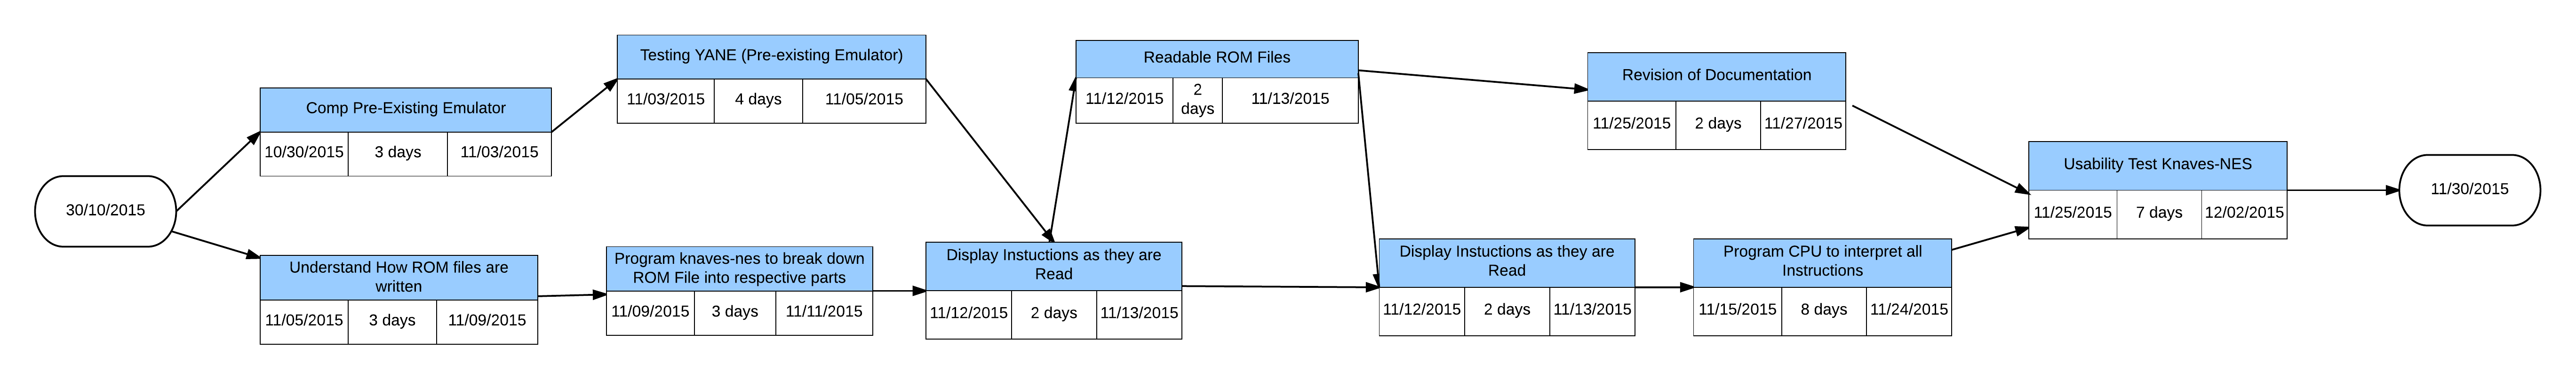
\includegraphics[width=180mm]{pert.png}
		\caption{Pert Chart for Knaves NES (pert.png in this folder)}
	\end{figure}

\section{Gantt Chart}
	\begin{figure}[H]
		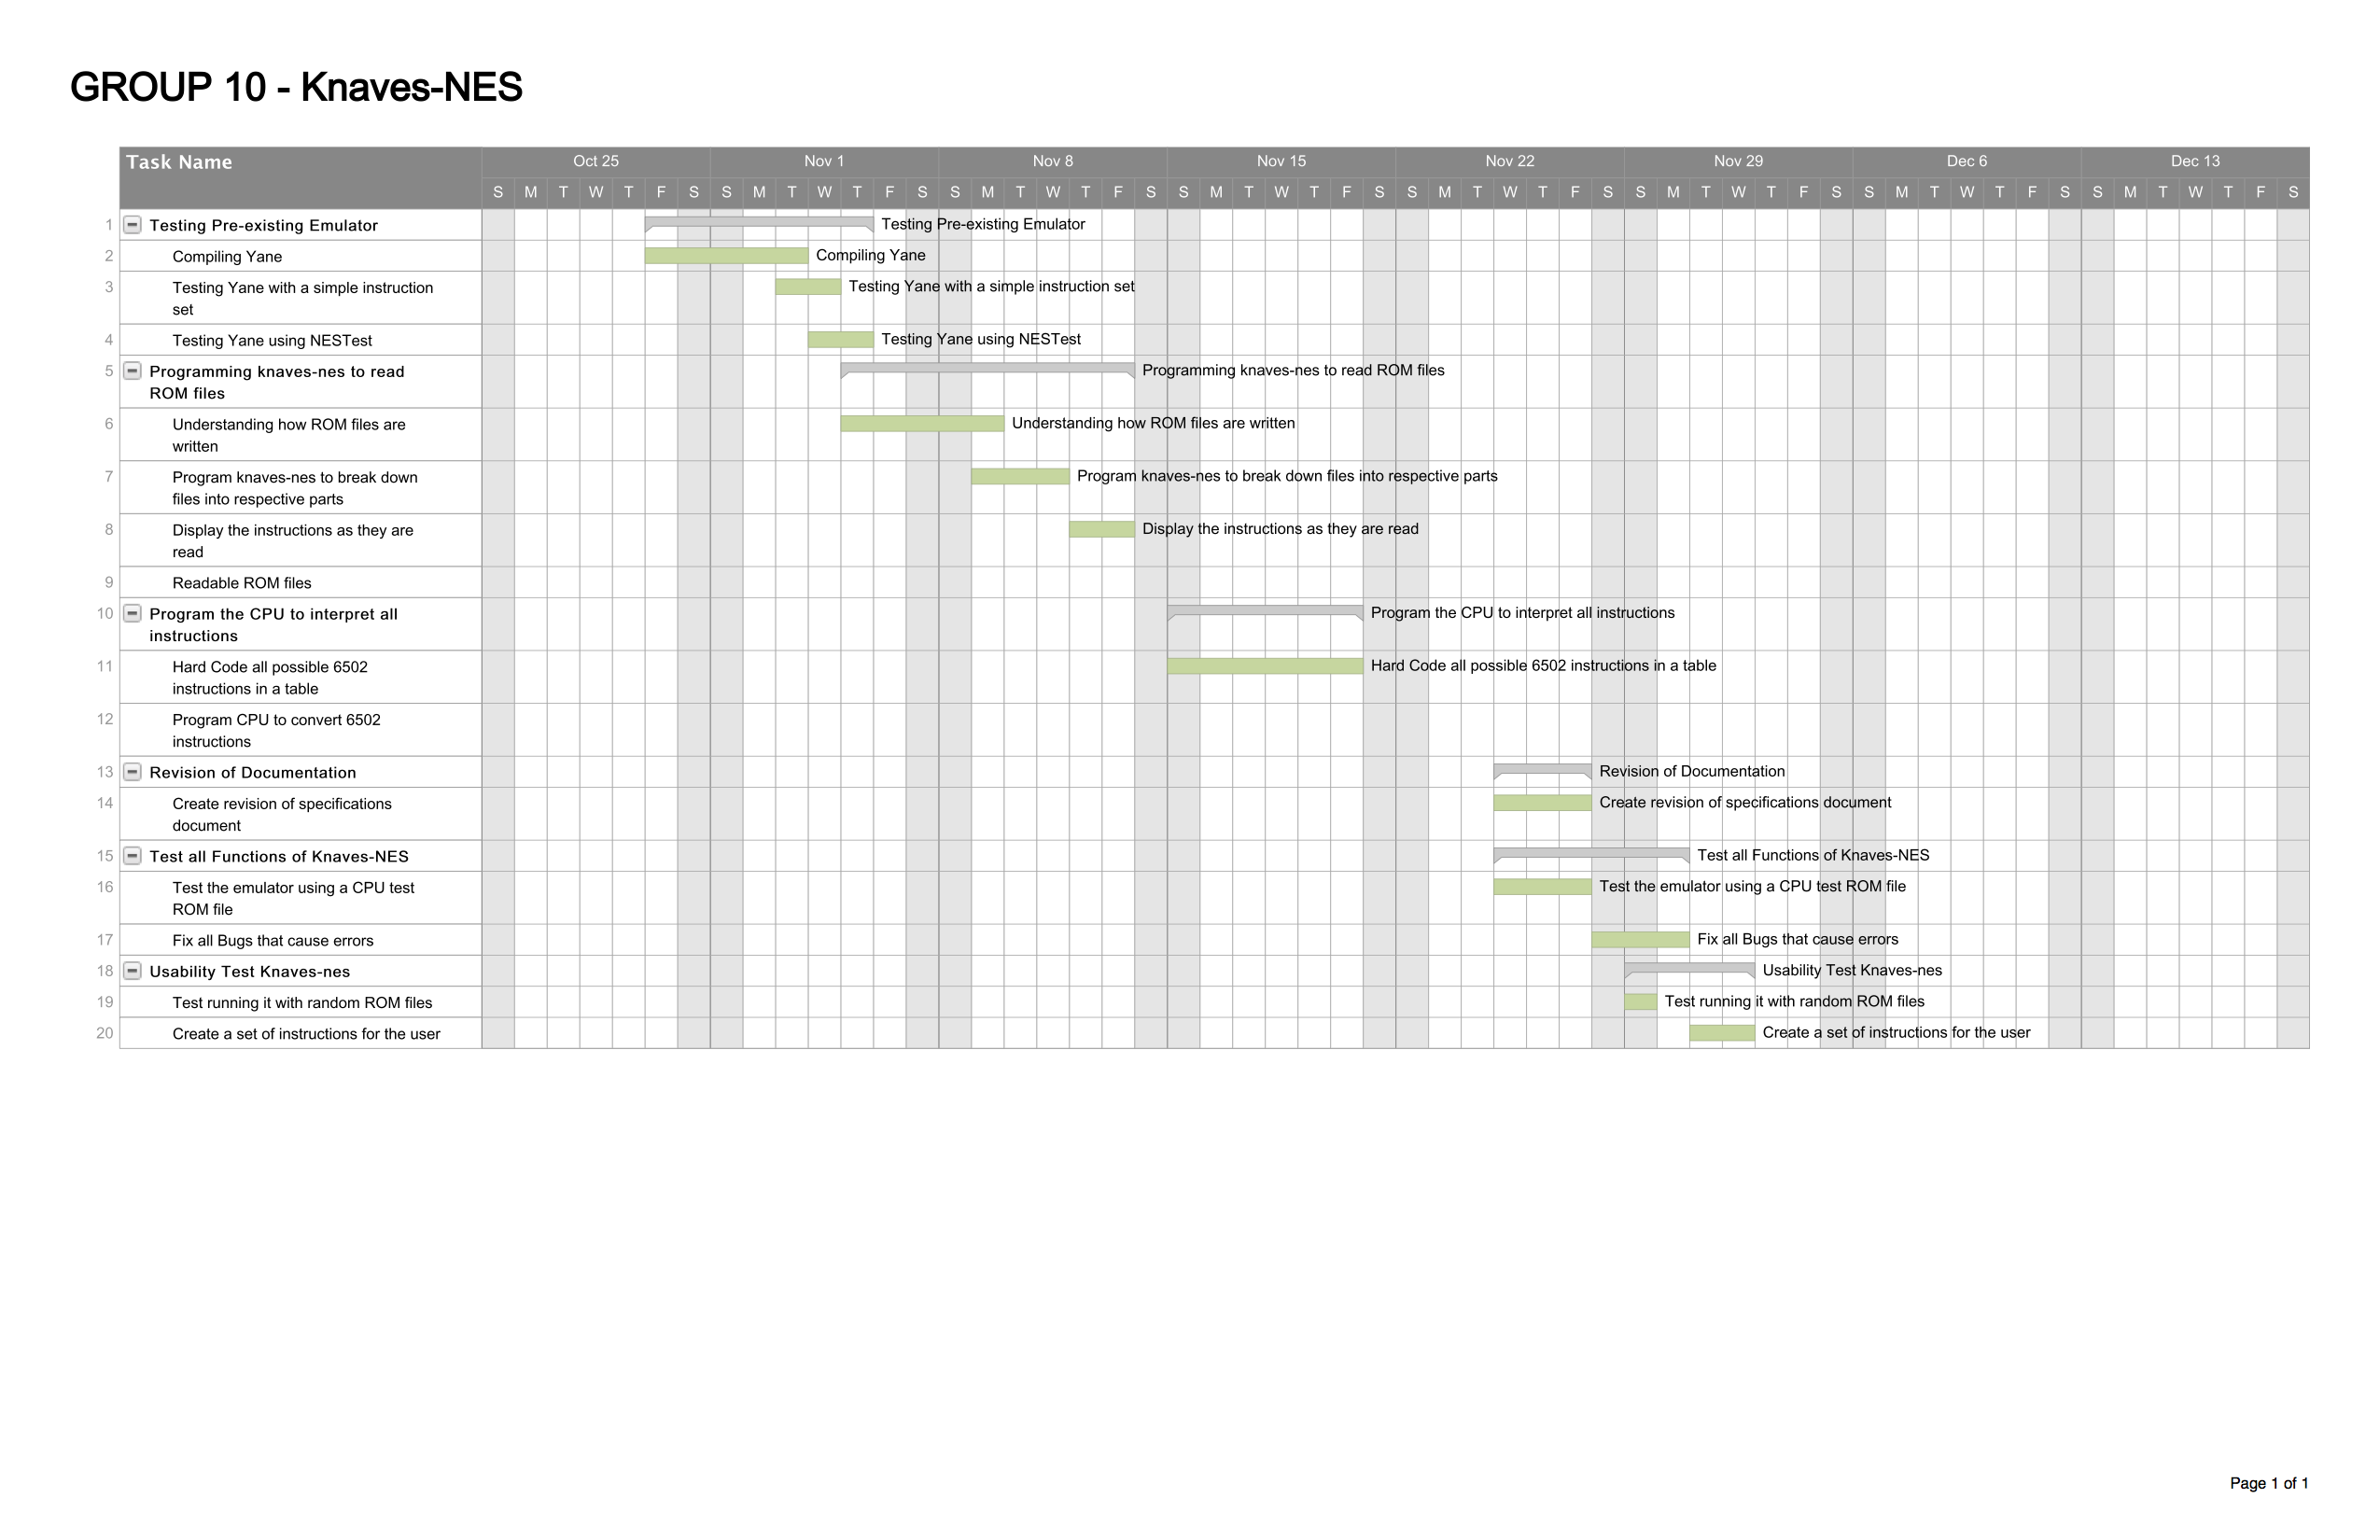
\includegraphics[width=180mm]{gantt.png}
		\caption{Gantt Chart for Knaves NES (gantt.png in this folder)}
	\end{figure}

\addcontentsline{toc}{section}{Version History}
% Start of the revision history table
\begin{versionhistory}
  \vhEntry{1.0}{Nov 5, 2015}{Niko Savas}{created}
  \vhEntry{2.0}{Nov 5, 2015}{Joe Crozier}{modified}

\end{versionhistory}

\end{document}